% =============================================================================
% Project : THE_PHILOSOPHY_OF_VIABILITY
% Book    : Book I — Ontology of Viability
% Book ID : VS.B01
%
% File    : 2_MAINMATTER/PART_I_IDENTITY_AND_MANIFESTATION/
%           CHAPTER_03_UNITY_AND_PLURALITY/sections/
%           section_05_plurality_and_composition.tex
%
% Section : Chapter 03, Section 05
% Title   : Plurality and Composition
%
% Purpose :
%   To examine the ontological relation between components,
%   compositional organization, wholes, and identity without
%   reducing identity to composition or inferring identity
%   plurality from component multiplicity.
%
% =============================================================================

\section{Plurality and Composition}
\label{sec:plurality-and-composition}

% -----------------------------------------------------------------------------
\subsection{The Ontological Problem of Composition}

Composition introduces a specific problem into the analysis
of unity and plurality. An existent may involve multiple
components that participate in an organized configuration.
The components may differ in their material constitution,
structural position, relations, determinations, or modes
of manifestation.

The presence of such components raises questions about
the ontological relation between the components and the
configuration in which they participate. It also raises
the question of whether the unity of that configuration
has implications for the identity attributed to it.

These questions must not be answered by counting components
alone. A plurality of components does not establish a
plurality of identities. Equally, the organization of
several components into one composition does not establish
that the composition possesses exactly one identity.

Composition and identity therefore require distinct
analyses. Their possible relation must be investigated
without presupposing that either the components or the
composed whole provide an exhaustive foundation for identity.

% -----------------------------------------------------------------------------
\subsection{Composition as an Organized Relation}

Composition is considered here as an ontological relation
through which multiple components participate in the
constitution of a more comprehensive configuration.
It is not merely the act of considering several elements
together, nor is every collection of elements necessarily
a composition in the relevant sense.

A composition may involve relations of arrangement,
organization, integration, dependence, or constitutive
participation. The specific relations involved determine
how the components belong to the configuration and how
their organization differs from an arbitrary grouping.

The concept of composition must nevertheless be distinguished
from the concept of identity. An organized composition
may be identifiable as a configuration under a specified
description without the ontological status of its identity
being settled.

Likewise, participation in a composition does not by itself
establish that a component loses every form of ontological
distinction. The components may remain differentiated
while participating in relations that constitute the whole.

Composition must therefore be examined as a relation
among constituents. It cannot be treated, without further
argument, as a complete explanation of the identity
of the resulting configuration.

% -----------------------------------------------------------------------------
\subsection{Plurality of Components and Plurality of Identities}

The plurality of components is not sufficient to establish
the plurality of identities. An existent may involve
several components while its identity remains unified
in a particular ontological respect. This possibility
blocks a direct inference from compositional multiplicity
to identity plurality.

The distinction can be expressed as follows:

\[
\text{Plurality of Components}
\not\Rightarrow
\text{Plurality of Identities}
\]

This expression does not establish that every composition
possesses one identity. It establishes only that the
number of components cannot serve as a direct measure
of the number of identities involved.

A component may participate in a composition without
being established as an independently distinct identity.
Conversely, a component may possess an identity that is
not reducible to its participation in the broader composition.
Whether either possibility obtains in a particular case
requires an independent ontological account.

The relation between components and identities must
therefore be examined without assuming a necessary
one-to-one correspondence.

% =============================================================================
% Project : THE_PHILOSOPHY_OF_VIABILITY
% Book    : Book I — Ontology of Viability
% Book ID : VS.B01
%
% File    : 4_ASSETS/tables/
%           VS.B01.P01.C03.S05.SS03.P012.TL01.components_composition_whole_and_identity.tex
%
% Asset   : TL01 — Components, Composition, Whole, and Identity
%
% Purpose :
%   To distinguish the principal ontological terms involved
%   in compositional analysis and to prevent unsupported
%   inferences from component multiplicity to identity.
%
% =============================================================================

\begin{table}[htbp]
\centering
\caption{Components, Composition, Whole, and Identity}
\label{tab:components-composition-whole-and-identity}

\small
\renewcommand{\arraystretch}{1.35}

\begin{tabular}{p{0.19\textwidth} p{0.34\textwidth} p{0.35\textwidth}}
\hline
\textbf{Term}
&
\textbf{Primary concern}
&
\textbf{What it does not establish by itself}
\\
\hline

Component
&
An element participating in a broader configuration.
&
That it possesses an independently distinct identity.
\\

Composition
&
The organized relations through which components
participate in a configuration.
&
That the resulting configuration possesses exactly
one identity.
\\

Aggregate
&
A plurality of elements considered together under
a grouping or unity criterion.
&
That the grouping constitutes a composition or
a distinct identity.
\\

Composed whole
&
A configuration considered through the organization
of its participating components.
&
That its identity is reducible to its components
or their arrangement.
\\

Structural organization
&
The positions and relations through which components
are organized.
&
That structural unity is equivalent to identity unity.
\\

Material constitution
&
The material elements and conditions involved
in the constitution of an existent.
&
That material continuity or integration determines
identity.
\\

Identity
&
The ontological unity or distinction attributable
at the level of identity.
&
That its status can be inferred solely from
component count or compositional organization.
\\

\hline
\end{tabular}

\end{table}

% =============================================================================
% END OF ASSET TL01
% =============================================================================

The table distinguishes the principal terms involved
in compositional analysis. It is not intended as an
exhaustive taxonomy. Its purpose is to prevent a conclusion
about identity from being inferred directly from a
description of components or their organization.

% -----------------------------------------------------------------------------
\subsection{Unity of Composition and Unity of Identity}

The unity of a composition does not automatically
establish the unity of identity. A composition may
exhibit extensive organization, structural integration,
or coordination among its components. These conditions
may warrant treating the components as one organized
configuration under a specified compositional respect.

Nevertheless, the unity of the configuration in that
respect does not settle whether its identity is singular,
plural, or related to the identities of its constituents
in another ontological manner.

The distinction can be expressed schematically:

\[
\text{Unity of Composition}
\not\Rightarrow
\text{Unity of Identity}
\]

This does not mean that composition is irrelevant to
identity. The organization of components may contribute
to conditions under which an identity is constituted,
maintained, or manifested. Such a contribution, however,
must be established rather than assumed.

The unity of composition and the unity of identity may
coincide in a particular existent. Their possible
coincidence does not make them conceptually equivalent,
nor does it establish a universal rule connecting them.

% -----------------------------------------------------------------------------
\subsection{Components and the Composed Whole}

The relation between components and a whole cannot
be adequately described through a simple opposition
between wholly independent parts and an entirely
self-contained whole.

Components may participate in the constitution of a
whole through relations that determine their arrangement,
dependence, and mutual contribution. At the same time,
the whole may possess determinations that cannot be
attributed to each component considered in isolation.

At least four possibilities require separate consideration:

\begin{enumerate}
    \item Components may retain distinct ontological
    determinations while participating in one composition.

    \item Components may acquire or enter into further
    determinations through their relations within
    a composition.

    \item The composed whole may exhibit determinations
    that are not attributable to the isolated components
    considered separately.

    \item The relation between components and whole may
    involve forms of dependence that cannot be described
    solely through spatial inclusion or material contact.
\end{enumerate}

These possibilities do not constitute a universal theory
of composition. They indicate that the relation between
components and whole must be examined through its
specific ontological conditions.

No conclusion about identity follows from the mere
presence of any one of these relations. In particular,
the attribution of a determination to the whole does
not automatically establish an additional identity,
and the distinction of a component does not automatically
establish an independent identity.

% -----------------------------------------------------------------------------
\subsection{Composition Without Homogeneity}

The formation of a composition does not necessarily
eliminate differences among its components. Components
may remain differentiated in their material, structural,
relational, or functional determinations while participating
in an organized whole.

Compositional unity therefore need not be understood
as the reduction of components to homogeneity. A whole
may be organized through differentiated contributions,
and the differences among its components may be relevant
to the organization of the composition.

Conversely, the preservation of differences among
components does not automatically negate the unity
of the composition. Difference and compositional unity
are not mutually exclusive in every respect.

This point must not, however, be transferred without
qualification to identity. The compatibility of internal
difference with compositional unity does not prove
identity unity. Whether differentiated components
belong to one identity or involve several identities
remains a distinct question.

% -----------------------------------------------------------------------------
\subsection{Composition and Material Constitution}

Material constitution may provide important conditions
for compositional relations. An existent may be constituted
through multiple material elements whose arrangement
and interaction contribute to its structure and
manifestation.

Material composition cannot, however, be treated as
an exhaustive definition of identity. The material
constituents of an existent may change while some
relevant ontological determinations remain preserved.
Conversely, the preservation of material constituents
does not by itself establish the preservation of identity.

Material continuity, material similarity, and material
integration are therefore insufficient as universal
criteria of identity unity or plurality. Their relevance
depends on the specific ontological question being examined.

This restriction does not imply that material constitution
is ontologically irrelevant. It means that the material
conditions of an existent must be distinguished from
the identity attributed to it. The significance of
material manifestation must be preserved without
reducing identity to material composition.

% -----------------------------------------------------------------------------
\subsection{Composition and Structural Organization}

Composition may involve structural organization through
which components occupy determinate positions and
participate in relations that constitute a configuration.
Such organization may distinguish one composition
from another and may be relevant to the conditions
under which a whole is constituted.

Structural distinction does not automatically establish
identity distinction. Two compositions may differ
structurally without that difference alone determining
whether they possess distinct identities. Conversely,
structural similarity does not establish that two
compositions share one identity.

Structural integration also cannot serve as a sufficient
criterion of identity unity. The fact that components
form a highly integrated structure does not establish,
without further argument, that the resulting whole
possesses only one identity.

The relation between composition and structure must
therefore be distinguished from the relation between
composition and identity. Structural organization
may be relevant to identity, but it cannot be treated
as an exhaustive substitute for identity itself.

% =============================================================================
% Project : THE_PHILOSOPHY_OF_VIABILITY
% Book    : Book I — Ontology of Viability
% Book ID : VS.B01
%
% File    : 4_ASSETS/diagrams/
%           VS.B01.P01.C03.S05.SS08.P032.DG01.components_composition_and_identity_relations.tex
%
% Asset   : DG01 — Components, Composition, and Identity Relations
%
% Purpose :
%   To represent the distinction between component plurality,
%   compositional organization, and identity without implying
%   that any one of these necessarily entails another.
%
% Requires (preamble):
%   \usepackage{tikz}
%   \usetikzlibrary{calc, positioning, fit}
% =============================================================================

\begin{figure}[htbp]
    \centering
    \hyphenpenalty=10000 \exhyphenpenalty=10000\relax  % no hyphenation inside diagram labels

    \begin{tikzpicture}[
        font=\small,
        node distance=0.4cm,
        % --- base box ---
        box/.style={
            draw, rounded corners=3pt, align=center,
            inner sep=6pt, line width=0.7pt
        },
        % --- node roles ---
        compbox/.style={box, text width=2.6cm, minimum height=1.1cm,
                        fill=blue!8, draw=blue!55!black},
        compositionbox/.style={box, text width=6.8cm, minimum height=1.5cm,
                               fill=blue!16, draw=blue!55!black},
        identitybox/.style={box, text width=6.8cm, minimum height=1.5cm,
                            dashed, fill=gray!10, draw=black!60},
        % --- frames and labels ---
        vsgroup/.style={draw=black!45, dashed, rounded corners=5pt,
                        inner sep=8pt, line width=0.5pt},
        grouplabel/.style={font=\footnotesize\itshape, text=black!75,
                           align=left},
        legendtext/.style={font=\scriptsize},
        % --- undirected lines (no arrowheads: no entailment, no priority) ---
        vsrel/.style={draw=black!70, line width=0.8pt},
        vslink/.style={draw=black!55, dashed, line width=0.7pt}
    ]

    % ---------------------------------------------------------------
    % Components (equal rank)
    % ---------------------------------------------------------------
    \node[compbox] (b) {Component B};
    \node[compbox, left=of b]  (a) {Component A};
    \node[compbox, right=of b] (c) {Component C};

    \node[vsgroup, fit=(a)(b)(c)] (comps) {};
    \node[grouplabel, anchor=south west] at (comps.north west) {
        Component plurality
    };

    % ---------------------------------------------------------------
    % Composition and identity
    % ---------------------------------------------------------------
    \node[compositionbox, below=1.1cm of comps] (whole) {
        \textbf{Composition}\\[3pt]
        Organized relations among components
    };
    \node[identitybox, below=1.1cm of whole] (id) {
        \textbf{Identity}\\[3pt]
        Unity or plurality requires identity-level grounds
    };

    % each component participates in the composition (straight, vertical)
    \draw[vsrel] (a.south) -- (a.south |- whole.north);
    \draw[vsrel] (b.south) -- (b.south |- whole.north);
    \draw[vsrel] (c.south) -- (c.south |- whole.north);

    % possible ontological relevance (not entailment)
    \draw[vslink] (whole) -- (id);

    % ---------------------------------------------------------------
    % Legend and interpretive constraint
    % ---------------------------------------------------------------
    \node[below=0.7cm of id, legendtext] (legend) {
        \tikz[baseline=-0.5ex]\draw[vsrel] (0,0) -- (0.6,0);~participation in an organized configuration
        \quad\quad
        \tikz[baseline=-0.5ex]\draw[vslink] (0,0) -- (0.6,0);~possible ontological relevance
    };

    \node[below=0.4cm of legend, text width=10.5cm, align=center,
          font=\footnotesize\itshape] {
        \textbf{Interpretive constraint:}
        The component-to-composition connections represent
        participation in an organized configuration. The
        composition-to-identity connection represents possible
        ontological relevance, not entailment. Component count
        and compositional unity do not determine identity number.
    };

    \end{tikzpicture}

    \caption{The distinct relations among components, composition, and identity}
    \label{fig:components-composition-and-identity-relations}
\end{figure}

% =============================================================================
% END OF ASSET DG01
% =============================================================================


The diagram distinguishes the relations among components,
composition, and identity. Its connections indicate
possible ontological relevance, not necessary entailment
or a fixed sequence of constitution.

% -----------------------------------------------------------------------------
\subsection{The Possibility of Multiple Identities Within a Composition}

The unity of a composition does not exclude the possibility
that multiple identities may be involved within it.
An organized whole may include components or subsystems
whose identity relations require independent examination.

However, the presence of differentiated components
or subsystems does not automatically establish that
each possesses a distinct identity. Such an attribution
requires grounds relevant to identity itself rather than
an inference from structural or functional differentiation.

A composition may therefore involve several determinations
at once: unity of composition, plurality of components,
differentiation of structural relations, and a possible
unity or plurality of identities. These determinations
concern different ontological respects and are not
contradictory merely because they coexist.

The possibility of multiple identities within a composition
must remain open. It must not be treated as an automatic
consequence of compositional multiplicity, nor excluded
by appealing to the unity of the composed whole.

% -----------------------------------------------------------------------------
\subsection{One Identity Across Compositional Transformation}

The relation between composition and identity also raises
the question of whether one identity may be associated
with different compositional configurations.

A composition may undergo changes in its components,
their arrangement, or their relations. Such changes
do not automatically establish the emergence of a new
identity. Nor does the preservation of a particular
composition automatically establish that the same
identity persists.

A reduction of identity to composition would tend to
treat every identity-relevant compositional change as
an identity change. An account that entirely separates
identity from composition, on the other hand, would
risk ignoring the possible constitutive significance
of compositional conditions.

Neither position can be accepted without further argument.
The relation must be examined in terms of the specific
conditions under which composition contributes to
identity constitution, manifestation, or distinction.

This inquiry must also distinguish compositional
transformation from identity persistence. The former
describes a change in the organization or constituents
of a composition; the latter concerns whether an identity
continues to obtain. One cannot be used as a substitute
for the other.

% -----------------------------------------------------------------------------
\subsection{Composition, Aggregate, and Identity}

Composition, aggregate, and identity must remain
conceptually distinct. An aggregate concerns a plurality
of elements considered together under some grouping
or unity criterion. A composition concerns relations
through which components participate in an organized
configuration. Identity concerns the ontological unity
or distinction attributable at the level of identity.

These concepts may refer to related aspects of an
existent, but they answer different questions. The
distinction can be summarized as follows:

\[
\begin{aligned}
\text{Aggregate} &\neq \text{Composition}
\\
\text{Composition} &\neq \text{Identity}
\\
\text{Unity of Composition} &\neq \text{Unity of Identity}
\\
\text{Plurality of Components} &\neq
\text{Plurality of Identities}
\end{aligned}
\]

The distinction between aggregate and composition
does not imply that every aggregate is wholly unorganized
or that every composition possesses a particular degree
of integration. It indicates that the relations through
which a whole is constituted must be specified before
conclusions about its ontological unity are drawn.

Similarly, the distinction between composition and
identity does not imply that identity is independent
of every compositional condition. It prevents composition
from being treated as sufficient, by itself, to determine
identity.

% -----------------------------------------------------------------------------
\subsection{The Limits of Compositional Reduction}

Compositional reduction occurs when identity is explained
entirely through components and their organization.
Such an account may provide important information
about the constitution of an existent, but it risks
assuming that a complete description of composition
is equivalent to a complete account of identity.

A description of components and their relations may
explain how a configuration is organized without
settling the ontological question of what identity
belongs to that configuration. The identification
of a composition is not yet an explanation of the
identity attributed to it.

The opposite reduction must also be avoided. Treating
identity as wholly independent of composition would
be premature where compositional conditions may
contribute to identity constitution, manifestation,
or distinction.

The appropriate position is therefore neither to
identify identity with composition nor to deny every
ontological relevance of composition. Composition
may be one dimension of the conditions relevant to
identity. Whether it constitutes, constrains, or
merely accompanies a particular identity relation
must be established through further analysis.

% -----------------------------------------------------------------------------
\subsection{Illustrative Case: Components and an Organized Configuration}

Consider a device assembled from several components.
The components may be distinguishable, replaceable,
or organized in different ways. Their arrangement
may constitute a functioning configuration, but the
mere fact that they form one assembled device does
not settle every question concerning identity.

The components may be considered individually, the
assembled configuration may be considered as a whole,
and the relations among the components may be examined
as a compositional organization. These are different
objects of analysis, even when they concern the same
concrete case.

% =============================================================================
% Project : THE_PHILOSOPHY_OF_VIABILITY
% Book    : Book I — Ontology of Viability
% Book ID : VS.B01
%
% File    : 4_ASSETS/illustrations/
%           VS.B01.P01.C03.S05.SS13.P047.IL01.components_and_composed_configuration.tex
%
% Asset   : IL01 — Components and Composed Configuration
%
% Purpose :
%   To illustrate the difference between distinguishable
%   components and their organization as a composed whole,
%   while leaving identity attribution unresolved.
%
% =============================================================================

\begin{figure}[htbp]
\centering

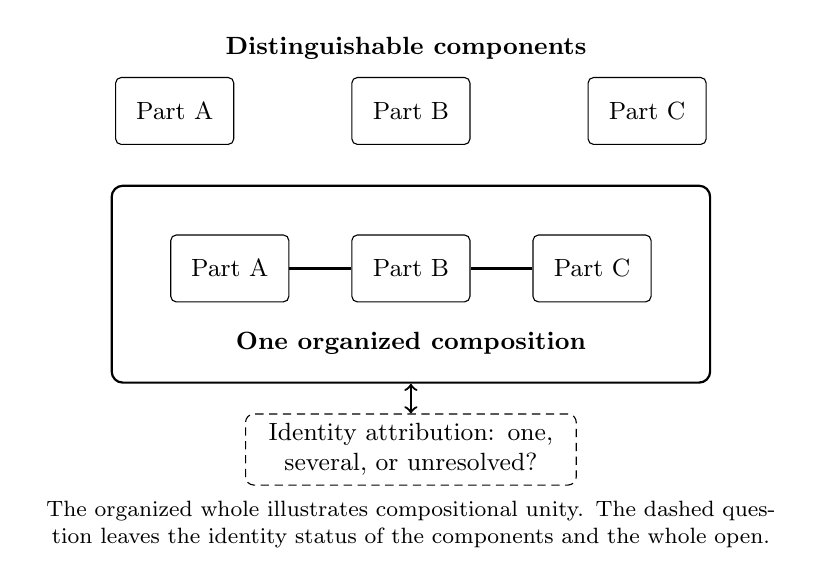
\begin{tikzpicture}[
    part/.style={
        draw,
        rounded corners=2pt,
        minimum width=1.5cm,
        minimum height=0.85cm,
        align=center,
        font=\small
    },
    whole/.style={
        draw,
        rounded corners=4pt,
        thick,
        minimum width=7.6cm,
        minimum height=2.5cm
    },
    question/.style={
        draw,
        densely dashed,
        rounded corners=3pt,
        minimum width=4.2cm,
        minimum height=0.9cm,
        align=center,
        text width=3.9cm,
        font=\small
    }
]

% Components considered separately
\node[part] (p1) at (-3.0,1.2) {Part A};
\node[part] (p2) at (0,1.2) {Part B};
\node[part] (p3) at (3.0,1.2) {Part C};

\node[align=center, font=\small\bfseries] at (0,2.0) {
    Distinguishable components
};

% Composed configuration
\node[whole] (frame) at (0,-1.0) {};

\node[part] (a) at (-2.3,-0.8) {Part A};
\node[part] (b) at (0,-0.8) {Part B};
\node[part] (c) at (2.3,-0.8) {Part C};

\draw[thick] (a) -- (b);
\draw[thick] (b) -- (c);

\node[font=\small\bfseries] at (0,-1.75) {
    One organized composition
};

% Identity question
\node[question] (identity) at (0,-3.1) {
    Identity attribution:
    one, several, or unresolved?
};

\draw[<->, thick] (frame.south) -- (identity.north);

\node[
    align=center,
    text width=9.5cm,
    font=\footnotesize
] at (0,-4.05) {
    The organized whole illustrates compositional unity.
    The dashed question leaves the identity status of
    the components and the whole open.
};

\end{tikzpicture}

\caption{Distinguishable components organized within one composition}
\label{fig:components-and-composed-configuration}

\end{figure}

% =============================================================================
% END OF ASSET IL01
% =============================================================================

The illustration is intended to clarify the distinction
between component multiplicity and compositional unity.
It does not establish whether the components or the
assembled configuration possess distinct identities.
Nor does it establish that the assembled whole constitutes
an additional identity. Those conclusions require
independent ontological grounds.

% -----------------------------------------------------------------------------
\subsection{The Relation to Unity and Plurality}

The analysis of composition clarifies that unity and
plurality cannot be attributed to an existent without
specifying their subject and respect. A composition
may be unified with respect to its organization while
remaining plural with respect to its components.

The same configuration may also raise questions of
identity unity or plurality that are not settled by
either of those descriptions. The unity of composition
and the plurality of components may coexist without
contradiction because they concern different
ontological determinations.

The relevant distinctions include:

\begin{itemize}
    \item Unity of composition and plurality of components.
    \item Unity of an aggregate and plurality of its constituents.
    \item Unity of identity and plurality of determinations.
    \item Unity of a broader configuration and possible
    plurality of identities.
\end{itemize}

These relations must not be collapsed into a single
opposition between the one and the many. The question
is not simply whether an existent is one or many. It
is necessary to determine what is one, what is many,
and whether the relevant claims concern components,
composition, aggregate, manifestation, or identity.

% -----------------------------------------------------------------------------
\subsection{Conclusion: Composition as Relevant but Non-Exclusive}

Composition is an important ontological dimension
in the examination of unity and plurality. It concerns
the relations through which multiple components
participate in an organized configuration.

Neither the plurality of components nor the unity
of their composition is sufficient, by itself, to
establish the plurality or unity of identity. Composition
may contribute to the conditions under which identity
is constituted or manifested, but it cannot be treated
as the exclusive foundation of identity.

Likewise, identity cannot be considered independent
of every compositional condition without further
argument. The ontological relation between composition
and identity must therefore be examined without
reducing either to the other.

The next section turns to the broader relation between
identity and multiplicity. It considers the different
forms of multiplicity that may occur within an existent
or across a plurality of existents, and examines why
multiplicity cannot be treated as synonymous with
plurality of identities.

% =============================================================================
% END OF SECTION 05 OF CHAPTER 03
% =============================================================================